
Este capítulo apresenta, inicialmente o sistema de escalonamento do BioNimbuZ em seus pormenores, a nível de classes e seus objetivos. Posteriormente, discorre sobre a implementação, mostrando alguns dos problemas encontrados durante o desenvolvimento e como eles foram solucionados. A terceira seção aborda a adição de tarefas que utilizam a \acrshort{GPU} no BioNimbuZ, e na última parte do capítulo são descritos os testes feitos e o resultado do novo escalonador.

\section{Sistema de Escalonamento do BioNimbuZ}

O serviço de escalonamento é implementado no BioNimbuZ como um serviço da Camada de Núcleo(veja a Figura \ref{Arquitetura}), de acordo com o subsistema mostrado na Figura \ref{SubsistemaDeEscalonamento}. A interface \textit{services} define métodos para inicialização, término de serviços e métodos para comunicação com o \textit{Zookeeper} \cite{Zookeeper}. A classe \textit{AbstractBioService} define funcionalidades comuns aos serviços do BioNimbuZ, em especial, comunicação entre as máquinas que compõem a plataforma e o padrão de projeto \textit{observer}, utilizado para notificação de eventos.
\begin{figure}[htbp]
	%	\centerline{\includegraphics[scale=0.04]{img/EscalonadorProposto.png}}
	\centerline{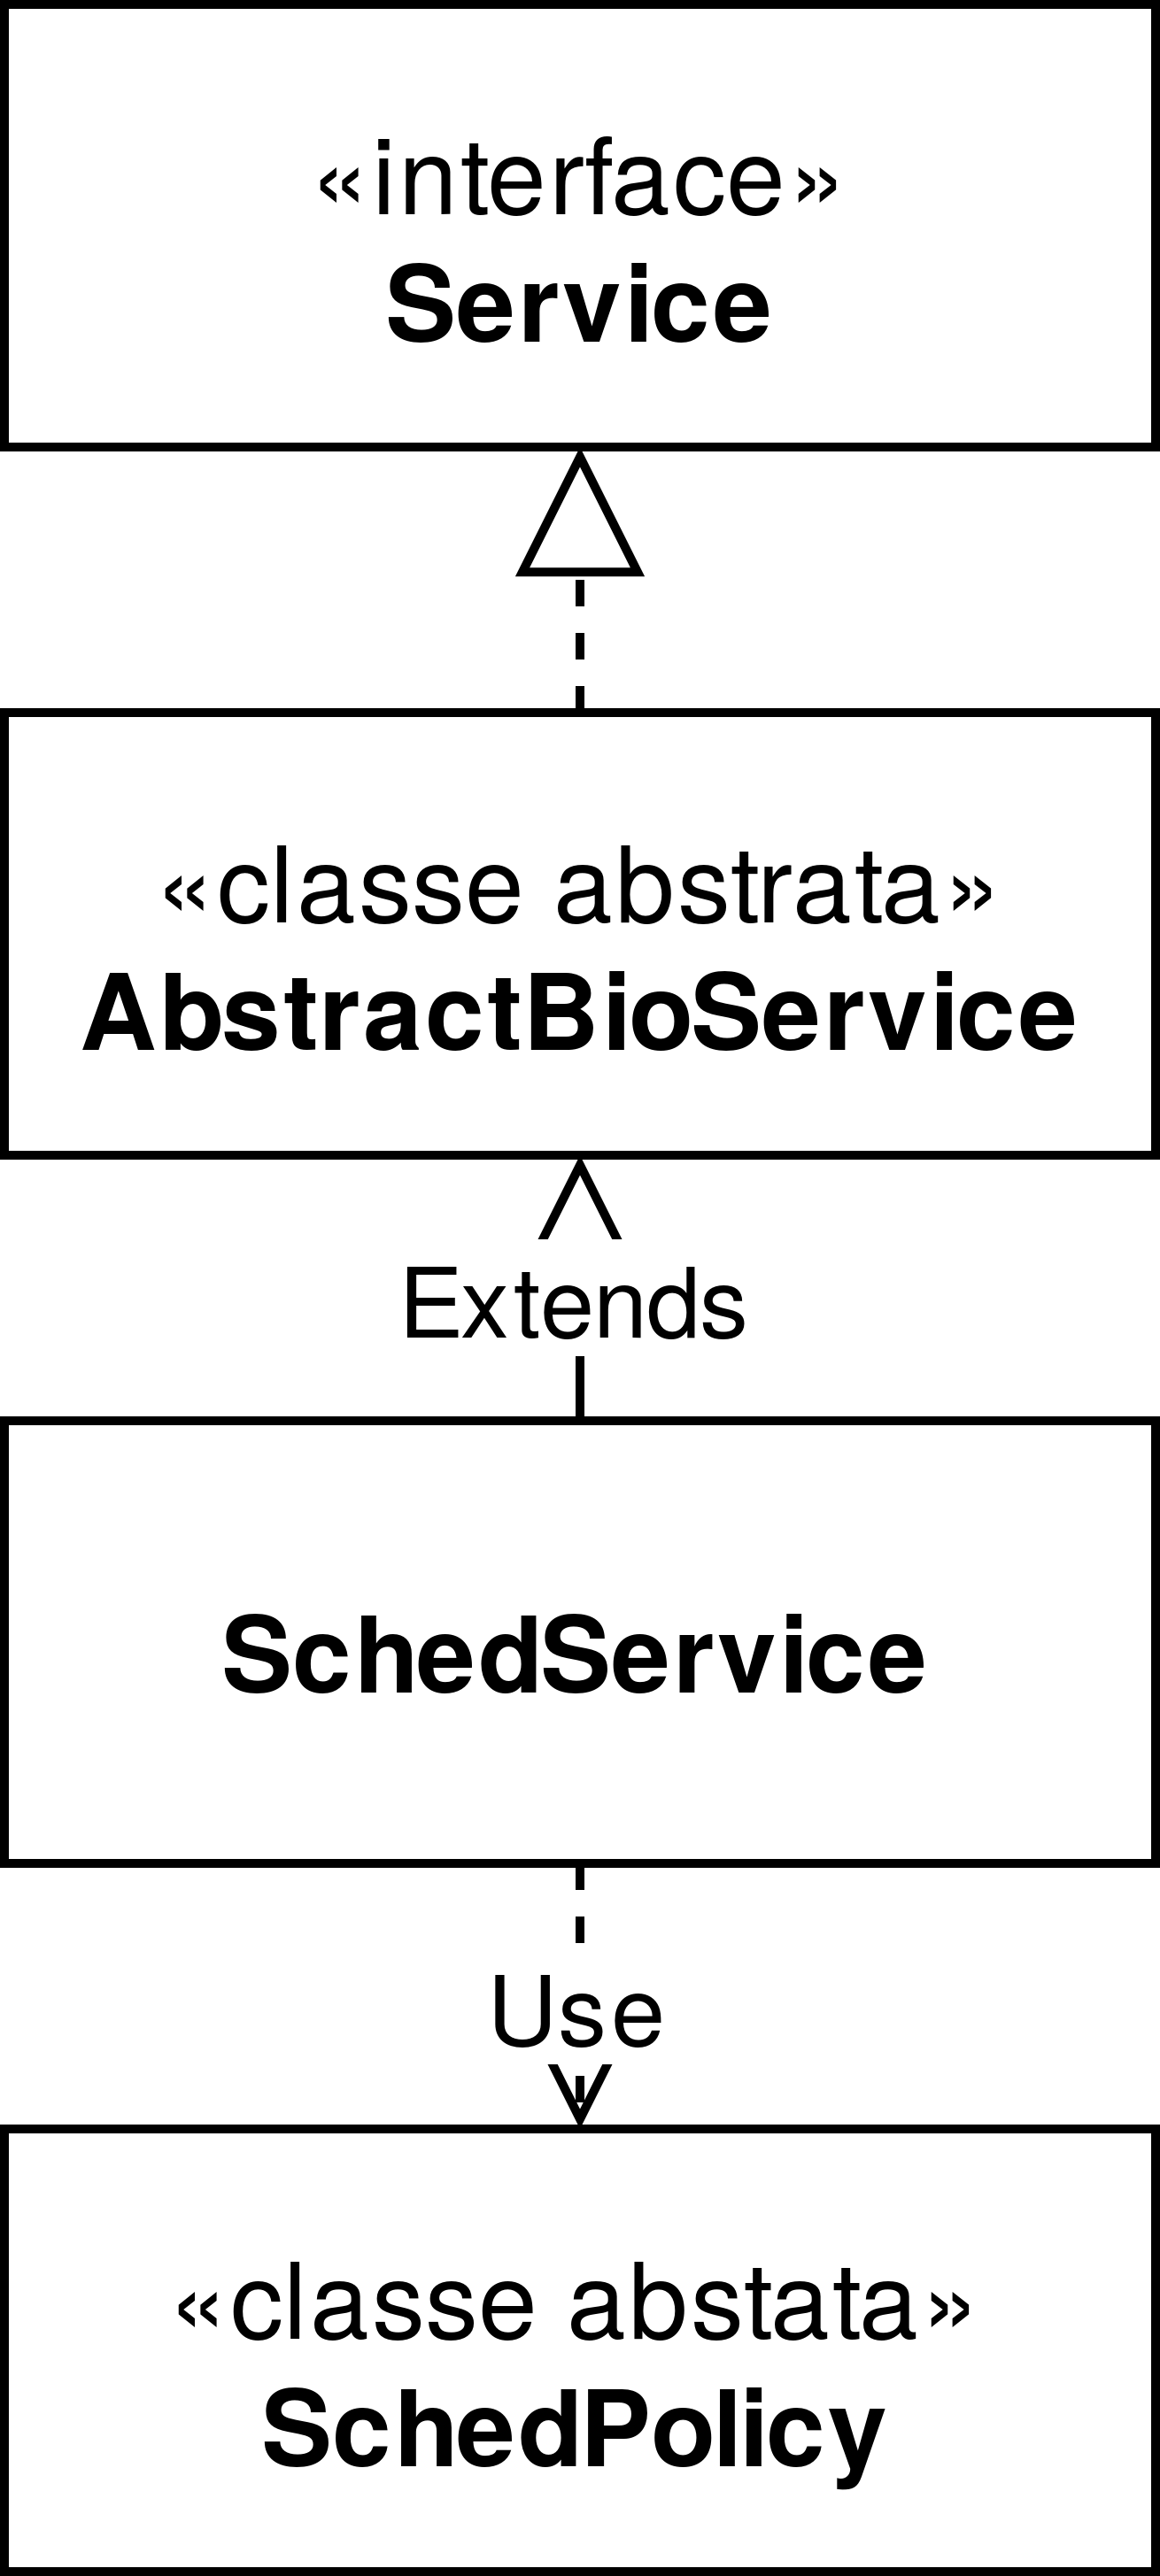
\includegraphics[width=2cm]{img/SubsistemaDeEscalonamento.png}}
	\caption{Subsistema de Escalonamento do BioNimbuZ}
	\label{SubsistemaDeEscalonamento}
\end{figure}

A classe \textit{SchedService} é a responsável por prover o serviço de escalonamento em si, entretanto, para permitir a existência de várias políticas de escalonamento, internamente ela utiliza instâncias da classe abstrata \textit{SchedPolicy}, que implementam cada uma das distintas políticas de escalonamento existentes. Conforme mostrado na Figura \ref{ArquiteturaAtual}.

Essas políticas de escalonamento são implementadas através da definição dos seguintes métodos herdados de \textit{SchedPolicy}:
\begin{itemize}
%	\item \textit{schedule}, que recebe como arguento uma lista de \textit{Jobs} para ser escalonado e retorna um mapeamento de \textit{Job} para um conjunto de máquinas as quais realizarão a computação.
	\item \textit{schedule}, que realiza o escalonamento inicial propriamente dito;
	\item \textit{relocate}, o qual realoca um processamento que está em execução;
	\item \textit{cancelJobEvent}, cujo objetivo é reportar ao escalonador o cancelamento de um \textit{job};
	\item \textit{jobDone}, que informa ao escalonador que um \textit{job} terminou.
\end{itemize}

\begin{figure}[htbp]
	\centerline{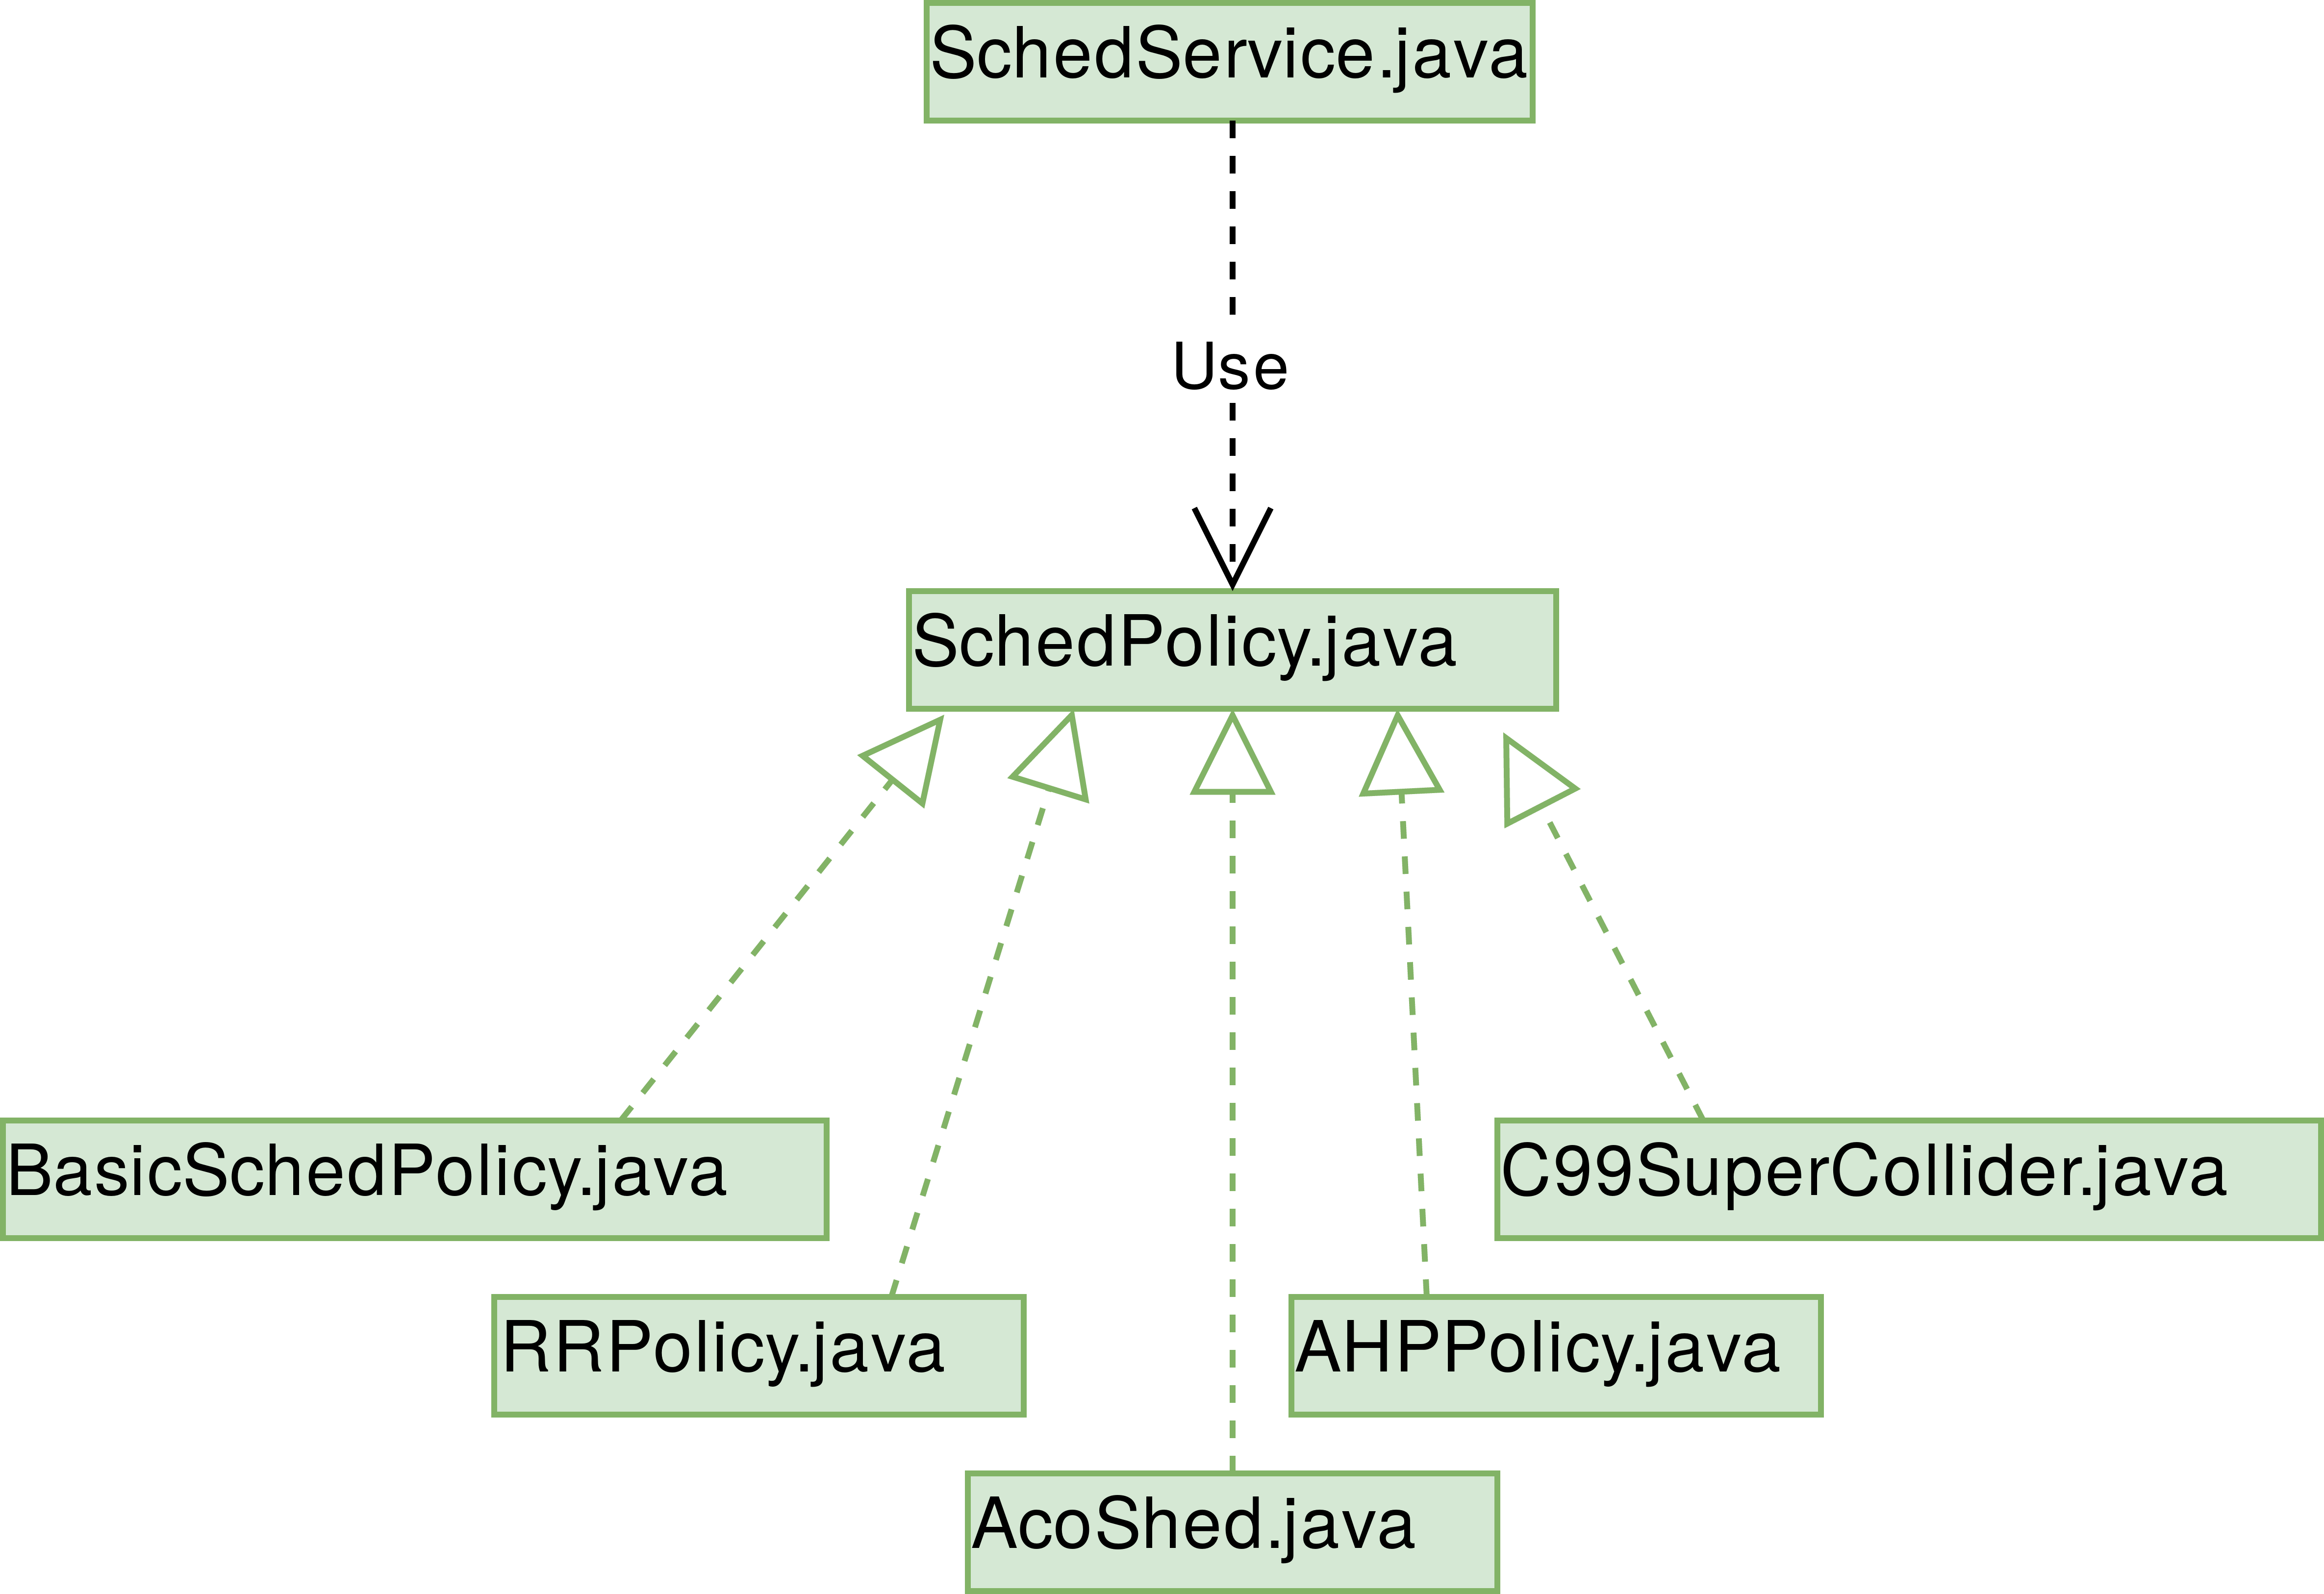
\includegraphics[width=12cm]{img/ArquiteturaAntesHoriz.png}}
	\caption{Subsistema de Escalonamento do BioNimbuZ}
	\label{ArquiteturaAtual}
\end{figure}


\section{Implementação do Escalonador}

Por motivos de familiaridade com a linguagem de programação, o escalonador proposto foi implementado em C++. Para ter compatibilidade com o resto do software, classes auxiliares, como a que representa os \textit{Jobs} e as \acrshort{VM}s instanciáveis tiveram equivalentes escritos em C++. Além disso, dois outros problemas surgiram, que foram como iniciar o escalonador C++, e como ele deve se comunicar com os demais componentes da plataforma. O primeiro problema foi resolvido através de pesquisa na \acrfull{API} do Java, utilizando as classes \textit{Process}\cite{JavaProcess}, \textit{Runtime}\cite{JavaRuntime} e \textit{ProcessBuilder}\cite{JavaProcessBuilder}, os quais permitem executar comandos de terminal, o que possibilitou a execução da parte C++ do escalonador.

O problema da comunicação do C++ com o Java é mais difícil, pois há várias formas de fazer. Por exemplo, o uso de classes \textit{wrappers} que usam \textit{handles}, que são objetos cujo objetivo é manipular estruturas que não são nativas da linguagem\cite{CppJavaHandle}. Uma outra forma documentada é através do uso do \acrfull{JNI}, que é uma outra forma existente no qual, através do uso de \textit{handles}, é chamar código C++ num programa Java\cite{CppJavaJNI}. Além disso, existem variações deste método utilizando bibliotecas que buscam simplificar o gerenciamento do \textit{handle}. Como as formas pesquisadas para fazer tal comunicação aparentam não chegar a um consenso, decidiu-se então utilizar formas mais genéricas de comunicação entre processos, onde então surgiu a ideia de usar \textit{sockets} para fazer a comunicação.

\textit{Socket} é uma abstração que sistemas operacionais fazem para permitir que programas tenham acesso à rede. \iffalse Os sistemas operacionais organizam os \textit{sockets} disponíveis e portas, essa organização de portas também é utilizada por protocolos de rede, \fi O sistema de portas permite diferenciar em um computador qual dos programas interessados está enviando ou deve receber a mensagem. %E um truque que pode ser feito usando a pilha de rede \acrshort{TCP/IP} é enviar mensagens para o próprio computador, através da interface de rede de \textit{loopback}. E esse é um método efetivo de comunicação entre processos distintos.

Uma vez decidido o uso de \textit{sockets} faltava decidir qual seria o protocolo da camada de rede e de transporte. Na camada de rede o principal protocolo existente é o \acrfull{IP}, entretanto, existem duas versões: o IPv4\cite{ipv4rfc} e o IPv6\cite{ipv6rfc}, sendo que o último é mais recente e permite um maior número de dispositivos na rede, por isso essa foi a versão utilizada na implementação. Quanto à camada de transporte, os candidatos eram o \acrshort{TCP}\cite{tcp_rfc} e o \acrshort{UDP}\cite{udp_rfc}. O \acrshort{TCP} provê uma série de garantias ao usuário dos pacotes que serão transmitidos pela rede ao custo de \textit{overhead}, mas como apenas será utilizado para comunicação em \textit{loopback}, o \acrshort{UDP} é mais simples e enxuto, sendo o escolhido como protocolo da camada de transporte neste trabalho.

\begin{figure}[htbp]
	\centerline{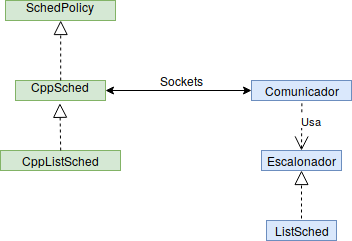
\includegraphics[scale=0.7]{img/Proposta.png}}
	\caption{Arquitetura de Classes do Escalonador Implementado.}
	\label{ArquiteturaProposta}
\end{figure}


Como pode ser observado na Figura \ref{ArquiteturaProposta}, para a implementação desse sistema de comunicação no BioNimbuZ, desenvolveu-se a classe abstrata \textit{CppSched} que herda de \textit{SchedPolicy}, responsável por fazer a inicialização do programa C++ e pelo \textit{handshake} entre os processos C++ e Java, permitindo que futuros escalonadores em C++ não precisem repetir este processo. Da classe \textit{CppSched} herda o método \textit{GetSchedPolicy}, utilizado para informar qual escalonador C++ deve ser utilizado.

\begin{figure}[htbp]
	\centerline{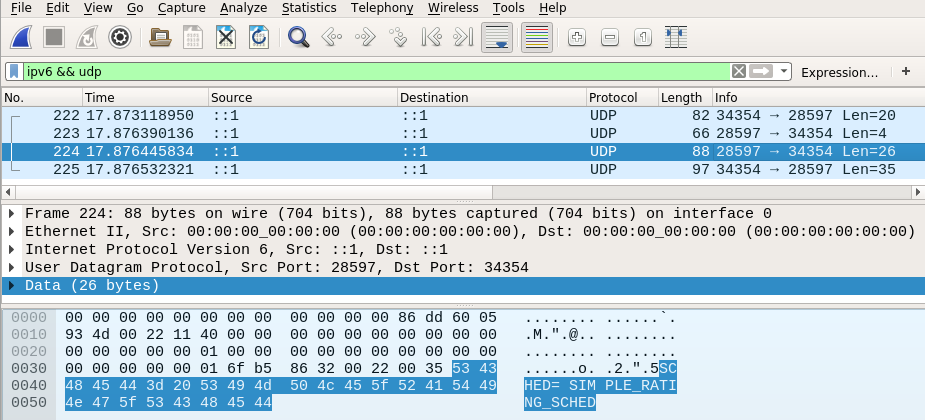
\includegraphics[width=13cm]{img/Handshake3.png}}
	\caption{Handshake entre a parte Java e C++ do Escalonador}
	\label{Handshake}
\end{figure}

O programa C++ é composto pela classe Comunicador, que inicializa seu \textit{socket} e inicia a conversa com o processo Java, cuja porta de comunicação é recebida pela linha de comando. Durante o \textit{handshake} é definido qual filho da classe virtual Escalonador será usado. Em prol da simplicidade e performance, buscou-se minimizar a comunicação entre os processos C++ e Java. Assim, após a inicialização, o processo C++ se comporta similarmente à um servidor \acrshort{DNS}\cite{dns_rfc}, ficando em espera por solicitações de escalonamento, e responde às requisições sem manter estado internamente.

\section{Implantação}

O escalonador foi inicialmente desenvolvido, utilizando apenas o subsistema de escalonamento do BioNimbuZ, para que testes fossem feitos com rapidez. Após testes que comprovaram o funcionamento do escalonador, como o da Figura \ref{Handshake}, utilizou-se uma máquina virtual para fazer a implantação do escalonador desenvolvido de volta ao BioNimbuZ, pois a instalação do BioNimbuZ requer instalação de programas que podem, mesmo que seja incomum, conflitar ou apresentar erros em iterações com o resto do sistema operacional. Um exemplo que ocorreu durante o desenvolvimento, foi uma atualização do sistema operacional, Debian\cite{Debian} Testing\cite{DebianTesting}, que causou erros em tempo de execução na \acrfull{IDE} Eclipse\cite{JavaEclipse}, relativos à interface gráfica. O mecanismo de \textit{snapshots} providos pelo software de gerenciamento de \acrshort{VM}s Virtualbox se revelou realmente útil nessa circunstância, como podemos ver na Figura 

\section{Uso de \acrshort{GPU} no BioNimbuZ}

%No início do projeto, imaginava-se que os \textit{workflows} existentes no BioNimbuZ seriam capazes de tirar proveito da \acrshort{GPU}, pressuposto que se revelou falso ao longo do desenvolvimento do projeto. Logo fez-se necessário procurar por programas de uso geral que utilizem a \acrshort{GPU}, uma atividade que se revelou simples. 
Para os testes foi escolhido o programa XMR-Stak\cite{xmr_stak}, um programa de mineração de criptomoedas, que são artefatos digitais desenvolvidos como meio de troca, que utilizam criptografia para prover segurança e integridade à transações\cite{crypto_currencies}. Esse software de mineração, em específico, foi escolhido pelo fato de ser software livre e por isso ter seu código fonte disponível publicamente, além de ser multiplataforma e ser capaz de minerar tanto em CPU quanto em GPU.

A mineiração de criptomoedas é a atividade de buscar \textit{nouces}, isto é, uma sequência aleatória de bytes, que quando inserido junto de um possível futuro bloco de uma \textit{blockchain}, que é uma lista distribuída para armazenamento de registros, numa função de \textit{hash} criptográfico, gera um \textit{hash} que atenda a algum critério de dificuldade, geralmente um valor específico no início. Quando é encontrado um \textit{digest}, uma saída da função de \textit{hash}, que atende ao criteírio, tal bloco é adicionado na \textit{blockchain}, e o responsável pela máquina que encontrou a resposta é recompensado em criptomoeda.



%A implementação da comunicação e sockets entre os processos 
 


